\documentclass[]{article}

\usepackage[italian]{babel}
\usepackage[margin=20mm, footskip = 20pt]{geometry}
\usepackage{array}
\usepackage{tabularx}
\usepackage{graphicx}
\usepackage{subfiles}
\usepackage{hyperref}
\usepackage{nameref}
\usepackage{titlesec}
\usepackage{longtable}
\usepackage[table]{xcolor}
\usepackage{titling}
\usepackage{lastpage}
\usepackage{ifthen}
\usepackage{calc}
\usepackage{soulutf8}
\usepackage{contour}
\usepackage{float}
\usepackage{fancyhdr}
\usepackage{multirow}
\usepackage{pgfgantt}
\usepackage{lscape}

\newcommand{\hr}{\par\vspace{-.1\ht\strutbox}\noindent\hrulefill\par}

\graphicspath{ {./}
	{./commons/res}
}

%--------------------------------------------------
% Comandi per inserire contenuto del documento
%--------------------------------------------------
\makeatletter

\newcommand\appendToGraphicsPath[1]{%
	\g@addto@macro\Ginput@path{{#1}}%
}

\newcommand{\setTitle}[1]{%
	\newcommand{\@phTitle}{#1}%
}
\newcommand{\phTitle}{\@phTitle}

\newcommand{\setDate}[1]{%
	\newcommand{\@phDate}{#1}%
}
\newcommand{\phDate}{\@phDate}

\newcommand{\setUso}[1]{%
	\newcommand{\@uso}{#1}%
}
\newcommand{\uso}{\@uso}

\newcommand{\setVersione}[1]{%
	\newcommand{\@versione}{#1}%
}
\newcommand{\versione}{\@versione}

\newcommand{\disabilitaVersione}{%
	\renewcommand{\setVersione}[1]{}%
	\renewcommand{\versione}{DISABILITATA}
}

\newcommand{\setResponsabile}[1]{%
	\newcommand{\@responsabile}{#1}%
}
\newcommand{\responsabile}{\@responsabile}

\newcommand{\setRedattori}[1]{%
	\newcommand{\@redattori}{#1}%
}
\newcommand{\redattori}{\@redattori}

\newcommand{\setVerificatori}[1]{%
	\newcommand{\@verificatori}{#1}%
}
\newcommand{\verificatori}{\@verificatori}

\newcommand{\setModifiche}[1]{%
	\newcommand{\@modifiche}{#1}%
}
\newcommand{\modifiche}{\@modifiche}

\makeatother 

%--------------------------------------------------
% Comandi per i documenti esterni e il glossario
%--------------------------------------------------

\newcommand{\dext}[1]{\textsc{#1\textsubscript{\textit{D}}}}

\newcommand{\glock}[1]{\textsc{#1\textsubscript{\textit{G}}}}

%--------------------------------------------------
% Comandi per impostare sottotitoli di quarto e quinto livello
%--------------------------------------------------

\setcounter{secnumdepth}{4}
\setcounter{tocdepth}{4}

\titleformat{\paragraph}
{\normalfont\normalsize\bfseries}{\theparagraph}{1em}{}
\titlespacing*{\paragraph}{0pt}{2.25ex plus 1ex minus .2ex}{1.5ex plus .2ex}

\titleformat{\subparagraph}
{\normalfont\normalsize\bfseries}{\thesubparagraph}{1em}{}
\titlespacing*{\subparagraph}{0pt}{1.75ex plus 1ex minus .2ex}{.75ex plus .1ex}

\appendToGraphicsPath{../../../commons/res/}

%------------------------------
%
% COMANDI DI CONFIGURAZIONE
%
%------------------------------

\setTitle{Verbale esterno \#3}

\setVersione{0.1.0}

\setDate{06-02-2021}

\setResponsabile{Valton Tahiraj}

\setRedattori{Alessandro Dindinelli}

\setVerificatori{Paolo Scanferlato}

\setUso{Esterno}

\setModifiche{
	0.1.0 & Paolo Scanferlato & Verificatore & 06-02-2021 & Verifica documento\\
	0.0.0 & Alessandro Dindinelli & Redattore & 01-02-2021 & Stesura iniziale}

\begin{document}
	
	% Direttive per la creazione del titolo tramite comando maketitle
\title{\huge \textsc{\phTitle{}} \\
	\vspace{11pt} \large \textsc{\phDate{}}}

\author{} % Non toccare
\date{} % Non toccare

%--------------------
% Frontespizio
%--------------------

% Logo del gruppo
\begin{figure}[t!]
	\centering
	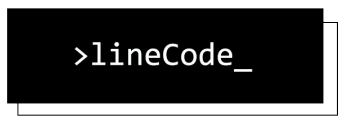
\includegraphics[width=20em]{lclong}
\end{figure}

% Titolo / Nome
\maketitle
\thispagestyle{empty}

% Dati specifici sul doc in forma tabulare
\begin{table}[ht]
	\begin{center}
		\label{tab:Dati sul documento}
		\begin{tabular}{r|l}
			\multicolumn{2}{c}{ \textsc{Dati sul documento} } \\
			\hline
			\textbf{Versione} & \versione{} \\
			\textbf{Uso} & \uso{}  \\
			\textbf{Redattori} & \redattori{} \\
			\textbf{Verificatori} & \verificatori{} \\
			\textbf{Responsabile} & \responsabile{} \\
			\textbf{Destinatari} & lineCode \\
								& prof.\ Vardanega Tullio \\		
								& prof.\ Cardin Riccardo \\
			\ifthenelse{\equal{\uso}{Esterno}}{
								& Sanmarco Informatica
			}{} \\
		\end{tabular}
	\end{center}
\end{table}

\newpage

\renewcommand{\arraystretch}{2} % allarga le righe con dello spazio sotto e sopra
\begin{longtable}[H]{>{\centering\bfseries}m{2cm} >{\centering}m{3.5cm} >{\centering}m{2.5cm} >{\centering}m{3cm} >{\centering\arraybackslash}m{5cm}}
	\rowcolor{lightgray}
	{\textbf{Versione}} & {\textbf{Nominativo}} & {\textbf{Ruolo}} & {\textbf{Data}} & {\textbf{Descrizione}}  \\
	\endfirsthead%
	\rowcolor{lightgray}
	{\textbf{Versione}} & {\textbf{Nominativo}}  & {\textbf{Ruolo}} & {\textbf{Data}} & {\textbf{Descrizione}}  \\
	\endhead%
	\modifiche{}%
\end{longtable}
	
	\newpage
	
	%--------------------------------
	%
	% IL CONTENUTO INIZIA DA QUI
	%
	%--------------------------------
	
	\section{Introduzione}
		\subsection{Luogo e data dell'incontro}
		\begin{itemize}
			\item \textbf{Modalità}: Telematica;
			\item \textbf{Software utilizzato}: Zoom;
			\item \textbf{Data}: 29 Dicembre 2020;
			\item \textbf{Ora di inizio}: 17:15;
			\item \textbf{Ora di fine}: 18:00.
		\end{itemize}
		
		\subsection{Presenze}
		\begin{itemize}
			\item \textbf{Presenti}: 
			\begin{itemize}
				\item Matteo Alba
				\item Giacomo Bulbarelli
				\item Alessandro Chimetto
				\item Alessandro Dindinelli
				\item Valton Tahiraj
			\end{itemize}
			\item \textbf{Assenti}:
			\begin{itemize}
				\item Lucia Fenu
				\item Paolo Scanferlato
			\end{itemize}
			\item \textbf{Partecipanti esterni}:
			\begin{itemize}
				\item prof. Tullio Vardanega
			\end{itemize}	
		\end{itemize}
		
		\subsection{Ordine del giorno}
		\begin{enumerate}
			\item Discussione casi d'uso;
			\item discussione requisiti.
		\end{enumerate}
\newpage	
	\section{Svolgimento}
	L'incontro è servito al gruppo per confrontarsi con il prof. Vardanega riguardo i commenti presenti nella correzione della RR.
	
		\subsection{Discussione casi d'uso}
		Commento: \textit{"I casi d’uso dell’AR sono troppo generici, e racchiudono al loro interno sotto-casi che rappresentano funzionalità molto differenti fra loro, rischiano di avere post-condizioni triviali e poco significative."}
		\newline
		È stato chiarito che il gruppo deve concentrarsi di più nel descrivere le pre e post condizioni dei casi d'uso, in modo da rendere più evidente quali possono essere dei sotto casi d'uso, e quali invece rappresentano scenari diversi tra loro.
				
	
		\subsection{Discussione requisiti}
		Commento: \textit{"I requisiti prestazionali pongono vincoli temporali, che dipendono anche da componenti esterne all’applicazione: riflettete su come sia possibile verificare il loro soddisfacimento."}
		\newline
		Sarà necessario ragionare su un ambiente significativo per il proponente per testare tali vincoli di tempo. \vspace{0.3cm}

		\noindent Commento: \textit{"Rivedere i requisiti di vincoli. Molti di essi insistono sul processo e pertanto sono requisiti di qualità."}
		\newline
		È stato fatto notare che bisogna capire il significato delle varie categorie di requisiti per evitare di sbagliare le suddivisioni. Riguardo il requisito che prevede il versionamento tramite \glock{Github}, è stato spiegato dal professore che se ciò è illustrato anche nelle \dext{Norme di progetto v1.0.0}, di fatto il requisito è già specificato e non serve ripeterlo.\vspace{0.3cm}
		
		\noindent Commento: \textit{"Solitamente non è possibile modificare l’identificativo che contraddistingue un oggetto di dominio."}
		\newline
		Si provvederà a modificare l'analisi fatta, in modo che l'amministratore possa inserire nuove unità con rispettivo ID, ma non modificarli.
		
	\newpage
	
	\section{Tabella delle decisioni}

\begin{table} [h!]
	\rowcolors{2}{gray!25}{gray!6}
	\begin{center}
		\begin{tabular} { m{2cm} m{14cm} }
			\rowcolor{lightgray}
			\textbf{ID} & \textbf{Decisione}\\
			VE03.1 & Verrà cancellato il requisito riguardante il versionamento tramite \glock{Github}.\\
			VE03.2 & Verranno ricontrollate e modificate opportunamente le pre e post condizioni dei casi d'uso.\\
			VE03.3 & Verrà tolto lo scenario in cui l'amministratore ha la possibilità di modificare le unità.
		\end{tabular}
	\end{center}
\end{table}
\end{document}

